\documentclass[a4paper]{article}
\usepackage{amsfonts}
\usepackage{amsmath}
\usepackage{amssymb}
\usepackage{graphicx}  
\usepackage{cancel}

\newcommand{\degree}{^{\circ}}
\newcommand{\cis}{\operatorname{cis}}
\newcommand{\Bgsin}{\operatorname{Bgsin}}
\newcommand{\Bgcos}{\operatorname{Bgcos}}
\newcommand{\Bgtan}{\operatorname{Bgtan}}
\newcommand{\limit}{\lim\limits}
\newcommand{\summation}{\displaystyle\sum}
\newcommand{\dom}{\operatorname{dom}}
\newcommand{\Int}{\displaystyle\int}

\begin{document}
  
\noindent \large Auteur: Rune Suy \\
\noindent \large Studierichting: Informatica\\
\noindent \large Oefeningenreeks 5I nr. 1.7\\

\medskip

\normalsize

$f(x) = x^3 + \dfrac{1}{12x} = \dfrac{12x^4+1}{12x}$ over $[1, 3]$\\

$f'(x) = \dfrac{12x \cdot 48x^3 - (12x^4 + 1) \cdot 12}{144x^2}$\\

$= \dfrac{36x^4-1}{12x^2}$\\

$f'(x)^2 = \dfrac{1296x^8 - 72x^4 + 1}{144x^2}$\\

$1 + f'(x)^2 = \dfrac{1296x^8 + 72x^4 + 1}{144x^2} = \left(\dfrac{36x^4+1}{12x^2}\right)^2$\\

$= \Int_1^3 \sqrt{\left(\dfrac{36x^4+1}{12x^2}\right)^2}dx =  \Int_1^3 \left(\dfrac{36x^4+1}{12x^2}\right)dx$\\

$= 3\left[\dfrac{x^3}{3}\right]_1^3 + \dfrac{1}{12}\left[\dfrac{-1}{x}\right]_1^3$\\

$= \dfrac{469}{18}$\\

\newpage

\begin{figure}[h]
\centering
    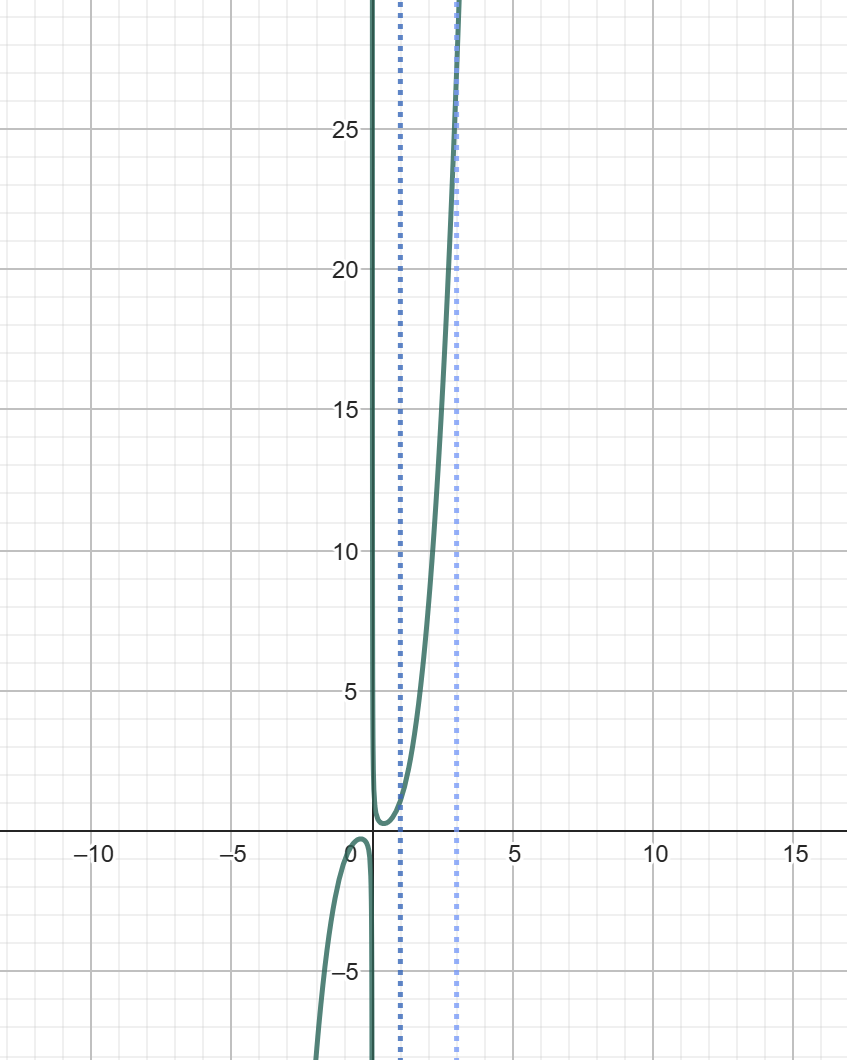
\includegraphics[width=\linewidth]{5I-1.7-rune.suy.INF.png}\\
\end{figure}

\begin{thebibliography}{999}
%\bibitem{a} Referentie
\end{thebibliography}
\end{document} 
